Para revisar la diferencia en eficiencia entre distintas implementaciones de \texttt{trafico}, consideramos las siguientes versiones del algoritmo de \textit{Dijkstra}: 1. sobre un \textit{min-heap}, por un costo temporal en $\Theta(m\log n)$\footnote{Ver cita \ref{foot_1}, sección 24.3.}; 2. utilizando un arreglo de manera \textit{ingenua} ---lo que permite actualizar la distancia a un vértice en tiempo constante, a cambio de un costo en $\Theta(n)$ para encontrar la próxima arista candidata--- con complejidad $\Theta(n^2)$; y 3. utilizando un \textit{queue}\footnote{En este caso, la estructura utilizada es la \textit{priority queue} de C$++$.} ``lazy'' ---en vez de agregar todos los nodos a la cola, estos se van colocando a medida que aparecen en la lista de adyacencia de los nodos candidatos y nunca se remueven---, por una complejidad temporal y espacial en $\Theta(m\log n)$.
% Para revisar la diferencia en eficiencia entre distintas implementaciones de \texttt{trafico} sobre el algoritmo de Djikstra consideramos tres algoritmos para solucionar este problema. El primero, al que llamaremos \textit{heap}, utiliza un heap para guardar todas las aristas y luego ir sacando las candidatas. y puede extraer el mínimo en tiempo constante y cambiar una clave en un razonable $\Theta(log(n))$. La complejidad temporal de este algoritmo es $\Theta(mlogn)$\footnote{Ver diapositivas de la clase 7, AED3}. Una segunda implementacion, a la que llamaremos \textit{ingenua}, funciona de la misma manera pero implementa el heap de forma ingenua, con un arreglo de costos y otro de valores. Esto permite cambiar claves en tiempo constante, pero a cambio encontrar el mínimo se hace en $Theta(n)$. La complejidad resultante es $Theta(n^2)$\footnote{Ver diapositivas de la clase 7, AED3}. Finalmente usamos \textit{queue}, una implementacion que utiliza la cola de prioridad del \textit{prelude} de C$++$ y un arreglo \textit{marcados} que indica si un elemento ya pasó por el queue o no. En vez de agregar todos los nodos a la cola como los otros dos algoritmos, este los va colocando en a medida que aparecen en la lista de adyacencia de los nodos candidatos. El arreglo \textit{marcados} evita que se repitan nodos. Tiene complejidad espacial de $Theta(mlogn)$\footnote{Ver diapositivas de la clase práctica 12 sobre camino mínimo}.

Teóricamente, \textit{ingenuo} debería ser más eficiente para instancias \textit{densas}, mientras que los otros dos resultan especialmente buenos para entradas \textit{ralas}. Sin embargo los tres algoritmos tienen distintos detalles de implementación que resultan interesantes de analizar empíricamente.%: Si bien \textit{ingenuo} es asintóticamente superior, realiza mucho trabajo de más al tener que recorrer la estructura entera cada vez para encontrar el mínimo. \textit{Queue} puede recorrer el mismo nodo varias veces si se ingresó a la cola en múltiples instancias, y además no tiene el costo de cambiar claves dentro del heap, pero como queue es una estructura de \textit{prelude} es probable que esté bien optimizada, en comparación con \textit{heap} que fue implementada "a mano".

Para cada una, realizamos una serie de tests para medir el tiempo de ejecución en función del tamaño de la entrada. Primero, evaluamos la influencia de la ``densidad'' del grafo para muestras aleatorias de tamaño $n = 15.000$, donde dejamos variar la cantidad de aristas $m$ en el rango $15.000$ y $11.247.750$ (caso completo) de a deciles. Luego, con muestras de tamaño $n = 10.000k$ y $m = 2n$, para cada $k$ natural en el rango $1 \leq k \leq 10$ ---para evaluar el desempeño en grafos \textit{ralos}--- y, finalmente, con muestras de tamaño $N = 10^6k$ para cada $k$ natural en el rango $1 \leq k \leq 10$, con $m = 2n$ ---para comparar, en mayor profundidad, el desempeño en grafos ralos de \textit{heap} y \textit{queue}---.

%Para ver empíricamente la diferencia en eficiencia entre estas tres implementaciones, realizamos una serie de evaluaciones, para cada una de estas implementaciones, respecto al tiempo de ejecución en función del tamaño de la entrada. Primero, evaluamos la influencia de la ``densidad'' del grafo para muestras aleatorias de tamaño $n = 15000$ $m = 15000 + 11247750 * k$ para cada $k$ natural  en el rango $1 \leq k \leq 10$, para cómo afecta la cantidad de aristas al tiempo de ejecución en cada algoritmo, luego con muestras de tamaño $N = 10000k$ para cada $k$ natural en el rango $1 \leq k \leq 10$, para observar el desempeño en grafos ralos. Y finalmente con muestras de tamaño $N = 1000000k$ para cada $k$ natural en el rango $1 \leq k \leq 10$, para comparar el desempeño en grafos ralos de \textit{heap} y \textit{queue}.

Efectuamos la primer evaluación diez veces para reducir la variación de los resultados y tomamos el promedio aritmético. Para la segunda evaluación lo hicimos $100$ veces, dado que los tiempos eran muy cortos.

Dado que nos interesa evaluar distintas implementaciones de \textit{dijkstra}, controlamos los parámetros de la función de la siguiente forma: elegimos $k = 0$, $s = 1$, $t = 2$ y definimos cada arista $x_i = (a_i,\ b_i,\ w_i)$, para todo $1 \leq  i \leq M$, $0 \leq w_i \leq 1000$ y $1 \leq a_i,\ b_i \leq n$ de manera aleatoria, tal que $a_i \neq b_i$ y $(a_i,\ b_i) \neq (a_j,\ b_j)$ para todo $1 \leq i,\ j \leq m$ e $i \neq j$.

%Notar que ninguna de estas decisiones afecta a la complejidad de las implementaciones de Djikstra. En efecto, el valor de K solo es relevante luego de haber corrido Djikstra, y S y T aleatorios no deberían tener efecto sobre la complejidad asintóticamente.

Las figuras \ref{grafico_1} y \ref{grafico_2} exponen los resultados de la experimentación. Los tres algoritmos parecen ---empíricamente--- mantener la misma complejidad, pero con distintas constantes asociadas. Nótese que, a pesar de su superioridad asintótica, \textit{ingenuo} resulta el más lento, incluso en el caso que ilustra un grafo completo. %Quizás tiene constantes demasiado grandes. Claramente \textit{queue} es la más rápida, quizás por la eficiencia de la implementación de la estructura.

\begin{figure}[!htbp]
    \subfloat{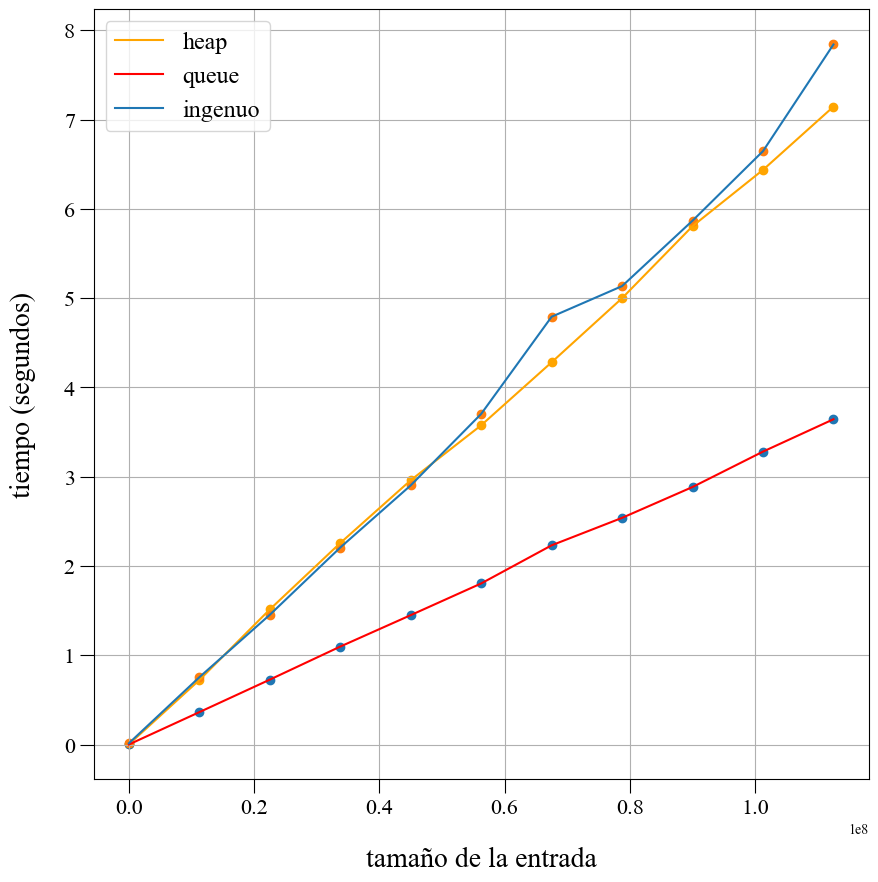
\includegraphics[scale=0.48, clip, trim={0.2cm 0 0 0}]{./files/src/.media/comparacion_triple.png}}

    \caption{Tiempo de ejecución de \texttt{trafico} en función del porcentaje de ``densidad'' del grafo de entrada, con $n = 15.000$, para las implementaciones \textit{ingenuo}, \textit{heap}, y \textit{queue}.}
    \label{grafico_1}
% \end{figure}

% % %\vspace{0.5em}
% \begin{figure}[!htbp]
    \subfloat{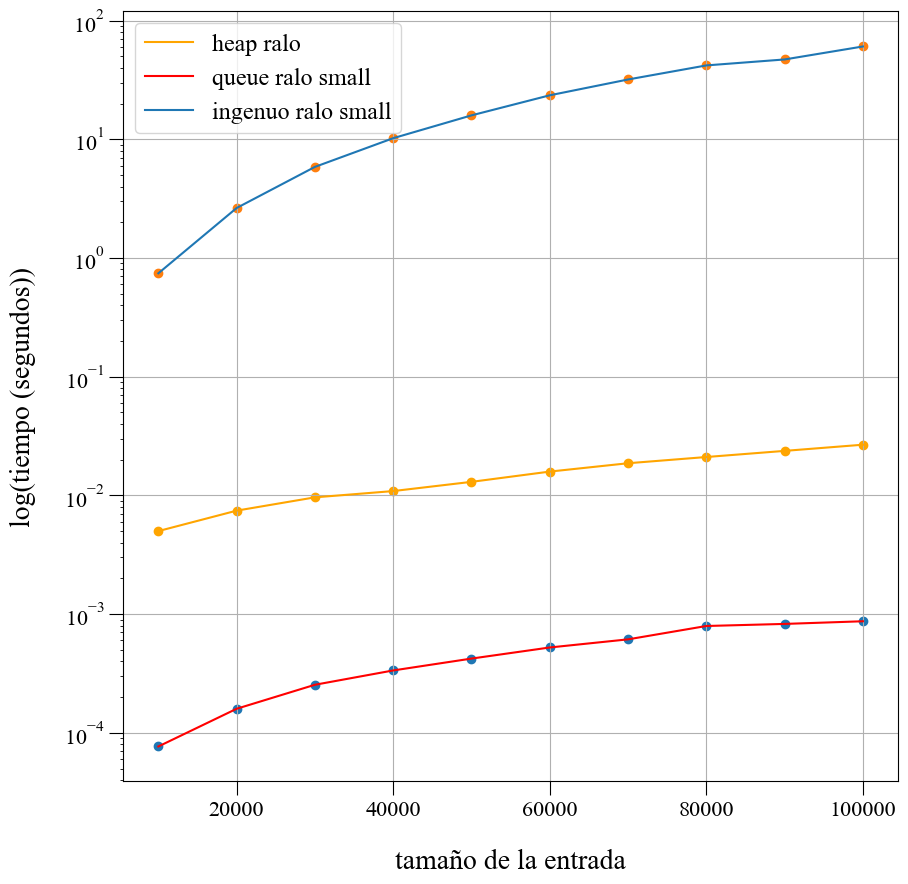
\includegraphics[scale=0.48, clip]{./files/src/.media/comparacion_rala_small.png}}
    %\hfill
    $\ \ \ \ $
    \subfloat{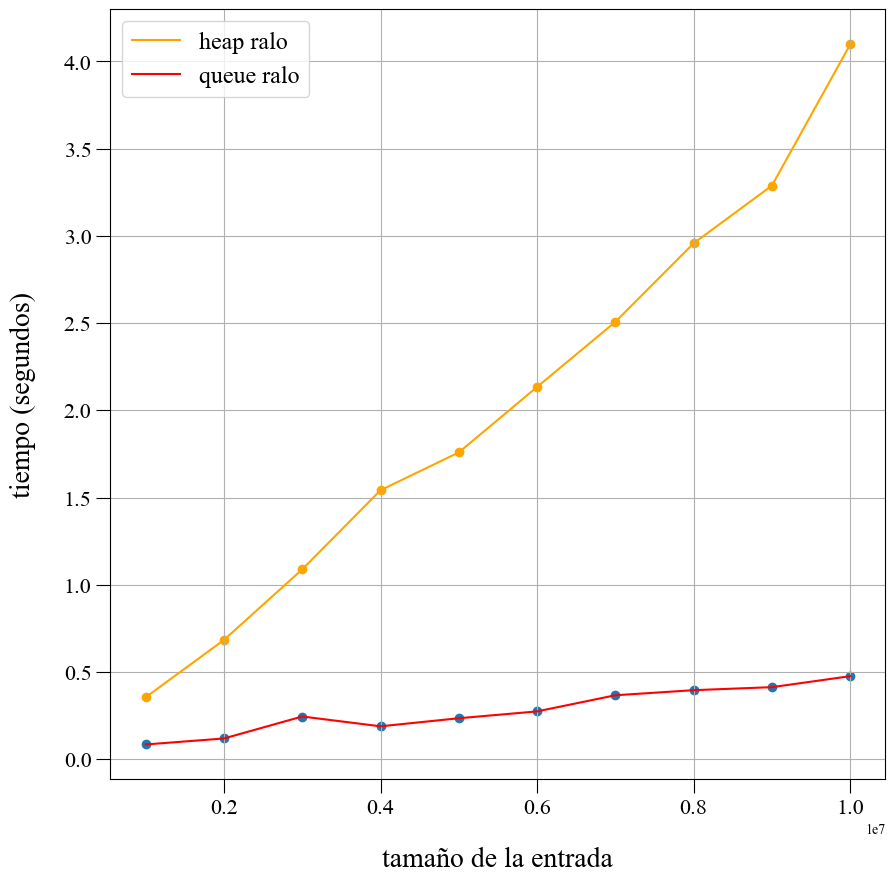
\includegraphics[scale=0.48, clip]{./files/src/.media/comparacion_rala_doble.png}}

    \caption{Izquierda: tiempo de ejecución de \texttt{trafico} en función del tamaño de entrada $n$ para los algoritmos \textit{ingenuo}, \textit{heap}, y \textit{queue}. Derecha: ejecución de \texttt{trafico} en función del tamaño de entrada $n$, con valores grandes, para \textit{heap} y \textit{queue}.}
    \label{grafico_2}
\end{figure}

Por su parte, es llamativo que \textit{queue} tenga mejor tiempo, ya que puede llegar a recorrer el mismo nodo varias veces si se ingresó a la cola en múltiples instancias. Sin embargo, consideramos que, como la estructura es parte de la biblioteca \textit{prelude} de C$++$, es probable que esté bien optimizada, en comparación con \textit{heap} que fue implementada ``a mano''.

%La figura \ref{grafico_2} expone los resultados de las experimentaciones en grafos \textit{ralos}. Notese que el algoritmo \textit{ingenuo} resultó extremadamente ineficiente en esta situación, por lo que se debieron utilizar instancias pequeñas para poder compararlo con los otros algoritmos. Como los tiempos de \textit{heap} y \textit{queue} son demasiado bajos en esta instancia, se comparan los dos solos con una entrada 100 veces más grande. De vuelta se nota una clara diferencia a favor del algoritmo \textit{queue}.